% =====================================================================
%  Sign-Aware Antithetic Coupling for Signed Gradient-Particle Methods
%  Coupled-estimation manuscript.  Separate from main-2.tex, which is
%  the two-speed compensation paper and is left unchanged.
% =====================================================================
\documentclass{article}
\usepackage{arxiv}
\usepackage[utf8]{inputenc}
\usepackage[T1]{fontenc}
\usepackage{amsmath,amssymb,amsthm,booktabs,graphicx,microtype}
\usepackage[numbers,sort&compress]{natbib}
\usepackage{doi,hyperref,xcolor,placeins,float}
\usepackage[ruled,lined,linesnumbered]{algorithm2e}
\usepackage{array}
\urlstyle{tt}

\theoremstyle{plain}
\newtheorem{proposition}{Proposition}[section]
\newtheorem{lemma}[proposition]{Lemma}
\newtheorem{corollary}[proposition]{Corollary}
\theoremstyle{definition}
\newtheorem{definition}[proposition]{Definition}
\theoremstyle{remark}
\newtheorem{remark}[proposition]{Remark}
\numberwithin{equation}{section}

\newcommand{\E}{\mathbb{E}}
\newcommand{\Var}{\operatorname{Var}}
\newcommand{\R}{\mathbb{R}}
\newcommand{\sgn}{\operatorname{sgn}}
\newcommand{\ind}{\mathbf{1}}
\newcommand{\Fil}{\mathcal{F}}
\newcommand{\refl}{\textnormal{\textsc{reflect}}}
\newcommand{\swi}{\textnormal{\textsc{switch}}}
\newcommand{\wit}{\textnormal{\textsc{within}}}
\newcommand{\pol}[1]{\textsc{#1}}
\graphicspath{{figures/}}
\raggedbottom

\title{Sign-Aware Antithetic Coupling for Signed Gradient-Particle Methods}
\author{Stephen Abkin \\
  Department of Mathematics \\
  Texas A\&M University \\
  College Station, TX, USA \\
  \texttt{stephen122204@tamu.edu}
  \And Prabir Daripa \\
  Department of Mathematics \\
  Texas A\&M University \\
  College Station, TX, USA \\
  \texttt{daripa@tamu.edu}}
\date{September 10, 2026}
\renewcommand{\shorttitle}{Sign-Aware Antithetic Coupling}
\renewcommand{\headeright}{Preprint}
\renewcommand{\undertitle}{Preprint}
\hypersetup{pdftitle={Sign-Aware Antithetic Coupling for Signed Gradient-Particle Methods},
  pdfauthor={Stephen Abkin, Prabir Daripa},colorlinks=true,linkcolor=blue,
  citecolor=blue,urlcolor=blue,hypertexnames=false}

\begin{document}
\maketitle
\thispagestyle{plain}

\begin{abstract}
Signed gradient-particle methods reconstruct a field by cumulatively summing
particle masses. Their sampling error depends on both particle positions and
mass signs, which makes the coupling of repeated simulations consequential.
We study an antithetic estimator that matches two replicas by spatial rank and
uses reflected Gaussian increments for like-sign masses and synchronous
increments for unlike-sign masses. The construction specializes established
coupling principles to transient field estimation without changing either
replica's discrete law. We prove an exact nonnegative reduction in conditional
integrated variance when the switch is applied at the final diffusion stage.
The identity identifies the relevant mass products and separations; it does not
imply a variance ordering for the complete nonlinear evolution.
For a two-pulse viscous Burgers problem, the proposed estimator has integrated
variance $0.739$ times that of within-sign pairing, with an approximate $95\%$
bootstrap interval $[0.682,0.801]$, and integrated mean squared error $0.819$
times as large. Its additional benefit is observed across fixed profiles,
observation times, and a cubic-flux test. In a held-out comparison, selected
plans using four and six trajectories respectively attain the same
expected-error target; the proposed estimator takes approximately $0.60$ of
the execution time of within-sign pairing. Heat and one-sign controls,
nonlinear observables, and bias-dominated regimes delimit these conclusions.
\end{abstract}

\keywords{gradient random walk \and signed particles \and antithetic coupling
  \and variance reduction \and viscous conservation laws \and Monte Carlo}

% =====================================================================
\section{Introduction}
\label{sec:intro}

Gradient-particle methods approximate the spatial derivative of a solution by a
signed particle measure and recover the field by cumulative summation. This
representation concentrates particles near steep gradients and supports a
mesh-free field reconstruction. Gradient random walks have been developed for
reaction--diffusion and viscous conservation equations
\citep{ghoniem1985,shermanpeskin1986,shermanpeskin1988,roberts1989,shermanmascagni1994}.
More recently, \citet{bertaglia2024} extended gradient-based Monte Carlo
constructions to relaxation approximations of hyperbolic conservation laws,
including systems. The present work concerns repeated estimation of a transient
field within an existing one-dimensional signed-particle solver.

The computational question is how to couple the randomness in two replicas.
Independent averaging reduces sampling variance but requires additional
trajectories. Antithetic sampling instead seeks a negative covariance between
the outputs of two runs with unchanged marginal laws
\citep{hammersley1956,glasserman2004}. In a signed cumulative reconstruction,
opposite masses reverse the response to a particle displacement. Reflection
of all matched Gaussian increments therefore need not give a favorable field
covariance, even when the particles are close in space.

We match particles by spatial rank and reflect their increments when the
matched masses have the same sign. When their signs differ, we use synchronous
increments. A natural alternative also uses the signs: pair particles within
each sign class and reflect every matched increment. The comparison between
these two sign-aware rules is central. It separates the benefit of retaining
spatial matching from the benefit already obtained by respecting mass signs.

\subsection{Related particle and coupling methods}
\label{sec:inherited}

The coupling principles have established antecedents.
\citet{nusken2018} formulate variance reduction through couplings with preserved
marginals. Their Proposition 54 and Corollaries 57--58 include
reflection/synchronization switches based on products of response-related
quantities; Section 5.2 describes repeated sorting and pairwise matching within
a collection of sampler copies. Their asymptotic variance analysis motivates
such constructions, but does not provide a finite-time variance comparison for
the signed interacting solver studied here. The choice of spatial rank and
mass sign is our specific realization of these ideas for a cumulative field
estimator. It requires no auxiliary equation, although computable switching
criteria also occur in the cited special cases.

Within the gradient-particle literature, \citet{lecot_rims2001} combines signed
cumulative reconstruction, spatial ordering, and quasi-random diffusion inputs
for a Burgers construction. A related treatment appears in
\citet{lecot2002}. This is the closest representation-specific precedent for
structuring the random inputs. Our randomized quasi-Monte Carlo comparison
adapts that diffusion strategy to the transport update used here; it is not a
reproduction of the complete published algorithm.

Recent QMC particle constructions also couple noise within an interacting
ensemble. \citet{benrached2024} prove weak convergence for additive-noise
McKean--Vlasov dynamics and develop an antithetic multilevel QMC estimator.
Their construction and regularity assumptions differ from our signed
rank-dependent solver. Together with array-RQMC work for a Fokker--Planck
particle model \citep{netterdon2026}, this places the diffusion adaptation below
within a broader literature; its result cannot rank QMC methods as a family.

\citet{bencheikhjourdain2019} study bias and antithetic sampling for mean-field
particle approximations. Their equation (3.1) couples a $2N$-particle system
with two $N$-particle systems to form a particle-number correction, an object
different from our same-size replica average. Related convergence and bias
analyses \citep{bossytalay1997,bossy2004,bossyjourdain2002,jourdain2000,bencheikh2020}
concern particular underlying particle schemes and assumptions. Preservation
of our baseline's law does not extend those theorems to a different
reconstruction or transport convention.

Variance reduction can also act through a control variate, conditional
expectation, or a modified particle representation
\citep{glasserman2004,baker2005,homolle2007,almohssen2010}.
We compare the coupling with two known-mean controls and conditional evaluation
of the last diffusion stage. These comparisons concern the selected estimators
and their implementations, rather than the best attainable performance of each
variance-reduction family.

\subsection{Contributions and organization}
\label{sec:contributions}

The contribution has three components. First, we specify a sign-aware
spatial-rank coupling for signed cumulative field estimation and establish
preservation of each replica's complete discrete law. This retains the
baseline expectation and allows its discretization bias to be studied
separately from the covariance introduced by pairing.
Second, we derive an exact final-stage variance identity and identify an
unconditional equality case when all masses have one sign. The identity is
local to the conditioned diffusion stage; a counterexample shows why an
unrestricted coordinatewise-monotonicity argument cannot supply the missing
nonlinear terminal comparison.
Third, we quantify the additional computational benefit over within-sign
pairing, alongside reflected sampling, controls, and a randomized
quasi-Monte Carlo adaptation. Fixed-profile experiments, two distinct held-out
target comparisons, and nonlinear observables establish the empirical scope.

The intended use is ensemble field estimation after a signed-particle solver
has been selected. We do not compare its efficiency with deterministic PDE
solvers. The numerical evidence is one-dimensional and scalar, and concerns
the mean-transport update defined below. In particular it does not establish
an advantage for sampled two-speed transport.

Section~\ref{sec:method} defines the update and estimators.
Section~\ref{sec:theory} gives their exact properties.
Section~\ref{sec:numerics} presents the comparisons and applicability tests,
followed by the discussion and conclusion. Appendices supply proofs, reference
and initialization details, and the statistical methodology.

\section{The solver, the estimators and the coupling}
\label{sec:method}

\subsection{Problem class and signed particle representation}

We consider the scalar viscous conservation law
\begin{equation}
 \partial_t u+\partial_x f(u)=\nu\partial_{xx}u,\qquad
 u(x,0)=u_0(x),\quad x\in\R,\quad 0<t\le T.
 \label{eq:pde}
\end{equation}
We take $f\in C^1(\R)$ and $\nu>0$, with initial data $u_0$ of
bounded variation whose derivative is integrable and whose limits
$u_\pm=\lim_{x\to\pm\infty}u_0(x)$ exist. The experiments use
$f(u)=u^2/2$ (viscous Burgers), $f(u)=u^3/3$, and $f\equiv 0$ (heat), the last
as a control in which the coupling acts without transport.

Differentiating \eqref{eq:pde} gives an equation for $w=\partial_x u$, which the
method represents by a signed atomic measure carried by $N$ particles,
\begin{equation}
  w^N(\cdot,t)=\sum_{i=1}^N m_i\,\delta_{X_i(t)},
  \qquad
  U^N(x,t)\;=\;u_-+\!\!\sum_{i:\,X_i(t)\le x}\!\! m_i .
  \label{eq:representation}
\end{equation}
The masses $m_i$ are fixed at initialisation and never change; only the
positions evolve. For the equal-far-field pulse profiles, we initialise deterministically, placing $N/2$ particles at
midpoint quantiles of the positive part of $u_0'$ and $N/2$ at those of the
negative part, each with $|m_i|=\mathrm{TV}(u_0)/N$
(Appendix~\ref{app:setup}). This gives equal counts and equal absolute mass per
sign class, and $\sum_i m_i=u_+-u_-$; for the smooth pulse profiles $u_+=u_-$, so
the total signed mass is zero. The one-sign control instead has nonzero total
signed mass and is initialized separately in Appendix~\ref{app:setup}. Zero total signed mass is a hypothesis of
Lemma~\ref{lem:wholeline} below and we flag where it is used.

\subsection{One step of a single replica}

Fix a step $h>0$, assume $K=T/h$ is an integer, and write $\sigma=\sqrt{2\nu h}$. A replica keeps
a state $(X,m,v)$ of positions, masses and carried velocities. Its storage
order is the most recent pre-diffusion rank order; after diffusion the positions
need not be sorted. Algorithm~\ref{alg:single} is one step: transport with the
velocity carried from the previous step, re-sort, read the new velocity off the
reconstructed field at the particle (inclusive of the particle's own mass), and
then diffuse.

\begin{algorithm}[H]
\caption{One step of a single replica (mean-transport gradient random walk)}
\label{alg:single}
\SetAlgoLined
\KwIn{state $(X,m,v)$ with associated entries, step $h$, viscosity $\nu$, flux derivative $f'$}
$X_i \leftarrow X_i + v_i\,h$ \qquad \tcp*[h]{transport with the carried velocity}\;
$\pi\leftarrow$ a stable sort of $X$; \quad $(X,m)\leftarrow(X_\pi,m_\pi)$\;
$v_i \leftarrow f'\!\bigl(u_- + \sum_{j\le i} m_j\bigr)$
  \tcp*{new carried velocity, inclusive cumulative sum}
draw $Z\sim\mathcal N(0,I_N)$ independent of the past;
  \quad $X_i \leftarrow X_i + \sigma Z_i$\;
\end{algorithm}

Three features of Algorithm~\ref{alg:single} matter later. The velocity is
computed \emph{after} the sort and \emph{before} the diffusion, and is used by
the \emph{next} transport, so it is part of the state and must stay associated with its particle until
used. At the subsequent sort the old velocity is discarded and recomputed; if
a state is reordered without recomputation, its velocity must be permuted too. The sort is stable, so ties are broken by prior order. And the
particles are not re-sorted between the diffusion and the following transport;
the next sort does that.

The velocity is evaluated from the rank-inclusive cumulative sum. At tied
positions this convention uses the stable particle order; it is not the value
of a field reconstruction that includes all co-located masses at once. The
same convention is used in every coupling. For Burgers, this is the
conditional-mean variant of the underlying two-speed implementation; here it
serves as a fixed baseline.

\subsection{Two replicas, a matching, and a multiplier}

Both replicas start from the same deterministic initial state. They are advanced
in lockstep. At stage $k$ let
\[
  S_k=\bigl(X^A,m^A,v^A,X^B,m^B,v^B\bigr)
\]
be the joint state \emph{after} the sort and the velocity update of
Algorithm~\ref{alg:single} and \emph{before} the diffusion, and let
$\Fil_k$ contain the complete joint history through this pre-diffusion stage, including all previous random draws.

\begin{definition}[admissible coupling]
\label{def:coupling}
An \emph{admissible coupling} is a rule that, at each stage $k$, selects a
bijection $\pi_k:\{1,\dots,N\}\to\{1,\dots,N\}$ and multipliers
$\varepsilon_k\in\{-1,+1\}^N$, both $\Fil_k$-measurable, draws
$Z^{(k)}\sim\mathcal N(0,I_N)$ independent of $\Fil_k$ and of all earlier draws,
and sets
\begin{equation}
  X^A_i \leftarrow X^A_i+\sigma Z^{(k)}_i,
  \qquad
  X^B_j \leftarrow X^B_j+\sigma\,\varepsilon_{k,j}\,Z^{(k)}_{\pi_k(j)} .
  \label{eq:coupling}
\end{equation}
\end{definition}

Three admissible couplings are compared throughout. All three use the same
$Z^{(k)}$ for replica $A$; they differ only in $(\pi_k,\varepsilon_k)$.

\begin{description}
\item[\refl{} (reflected pairing).] $\pi_k=\mathrm{id}$ and
  $\varepsilon_{k,j}=-1$. Matched by spatial rank, antithetic increments. This
  is the natural default.
\item[\swi{} (sign-switched pairing), the construction studied here.]
  $\pi_k=\mathrm{id}$ and
  \begin{equation}
    \varepsilon_{k,j}=-\,\sgn\!\bigl(m^A_j\bigr)\,\sgn\!\bigl(m^B_j\bigr),
    \label{eq:switch}
  \end{equation}
  so a matched pair with like masses is reflected and a matched pair with
  unlike masses is synchronised.
\item[\wit{} (within-sign pairing).] $\pi_k$ maps the $r$-th particle of sign
  $s$ in $B$ to the $r$-th particle of sign $s$ in $A$, for $s\in\{+,-\}$, and
  $\varepsilon_{k,j}=-1$. No matched pair ever has unlike masses.
\end{description}

\begin{algorithm}[H]
\caption{Coupled advance of two replicas}
\label{alg:pair}
\SetAlgoLined
\KwIn{common initial state $(X^0,m^0)$ sorted by position, $u_-$, steps $K$,
      step $h$, viscosity $\nu$, flux derivative $f'$, policy
      $\in\{\refl,\swi,\wit\}$}
$(X^A,m^A)\leftarrow(X^0,m^0)$; \quad $(X^B,m^B)\leftarrow(X^0,m^0)$;
  \quad $\sigma\leftarrow\sqrt{2\nu h}$\;
$v^A_i\leftarrow f'\!\bigl(u_-+\sum_{j\le i}m^A_j\bigr)$; \quad $v^B\leftarrow v^A$\;
\For{$k=0,\dots,K-1$}{
  $X^A_i\leftarrow X^A_i+v^A_ih$; \quad stable-sort $(X^A,m^A)$ by $X^A$; \quad
    $v^A_i\leftarrow f'\!\bigl(u_-+\sum_{j\le i}m^A_j\bigr)$\;
  $X^B_i\leftarrow X^B_i+v^B_ih$; \quad stable-sort $(X^B,m^B)$ by $X^B$; \quad
    $v^B_i\leftarrow f'\!\bigl(u_-+\sum_{j\le i}m^B_j\bigr)$\;
  \uIf{policy $=\refl$}{$\pi\leftarrow\mathrm{id}$; \quad $\varepsilon_j\leftarrow-1$\;}
  \uElseIf{policy $=\swi$}{$\pi\leftarrow\mathrm{id}$; \quad
    $\varepsilon_j\leftarrow-\sgn(m^A_j)\sgn(m^B_j)$\;}
  \Else(\tcp*[h]{$\wit$}){\ForEach{$s\in\{+1,-1\}$}{
      $I_s\leftarrow\{i:\sgn(m^A_i)=s\}$, $J_s\leftarrow\{j:\sgn(m^B_j)=s\}$,
        both in increasing order\;
      assert $|I_s|=|J_s|$; $\pi(J_s[r])\leftarrow I_s[r]$ for $r=1,\dots,|I_s|$;
        \quad $\varepsilon\leftarrow-1$ on those $j$\;
      }}
  draw $Z\sim\mathcal N(0,I_N)$ \tcp*{fresh, independent of the joint history}
  $X^A_i\leftarrow X^A_i+\sigma Z_i$; \quad
  $X^B_j\leftarrow X^B_j+\sigma\varepsilon_jZ_{\pi(j)}$\;
}
\KwOut{$(X^A,m^A)$, $(X^B,m^B)$; fields by \eqref{eq:representation} and the
       pair mean by \eqref{eq:est-pair}}
\end{algorithm}

Algorithm~\ref{alg:pair} is implemented by the shared coupling stepper in the
accompanying repository. Its Burgers trajectories are checked against the
conditional-mean baseline using prescribed draws. Drawing the fresh vector
before or after evaluating the state-dependent rule gives the same algorithm
provided the rule does not inspect that vector.

Figure~\ref{fig:construction} shows the two matchings on one paired state.
\wit{} buys the absence of unlike-sign pairs at the price of matching partners
that can be far apart in space; \swi{} keeps the spatially adjacent partners
and moves the sign logic into the multiplier.

\begin{figure}[htbp]
\centering
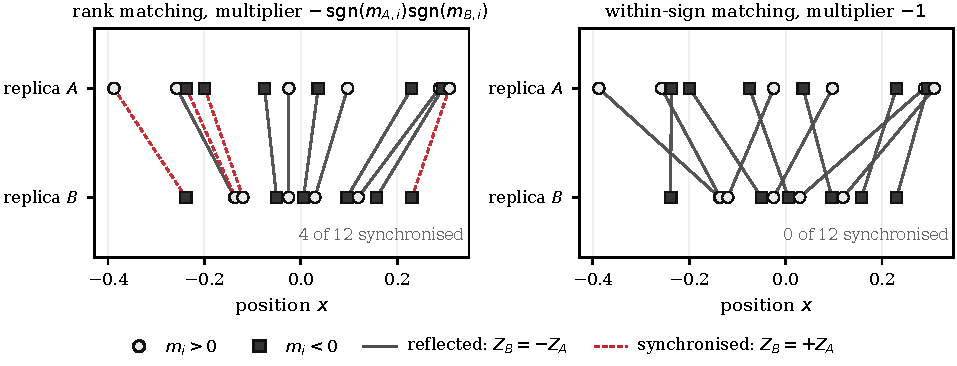
\includegraphics[width=\textwidth]{fig1_construction.pdf}
\caption{The two matchings on the same paired state, for the interleaved-sign
configuration just before the tenth diffusion stage with $N=12$ (regenerated by
\texttt{analysis/make\_figures.py}; state archived as
\texttt{analysis/fig1\_state.npz}). Left: rank matching pairs spatially
particles of equal rank; unlike-sign pairs are synchronised rather than reflected. Right: within-sign matching never
produces an unlike-sign pair, but its partners are further apart. Both rules
are bijections measurable with respect to the pre-diffusion joint state, so
both preserve each replica's marginal law (Proposition~\ref{prop:law}).}
\label{fig:construction}
\end{figure}

\paragraph{Implementation requirements.}
(i) The draw $Z^{(k)}$ must be \emph{fresh} at every stage and independent of
the complete joint pre-stage history, including both replicas' masses and
carried velocities; reusing one coordinate for two particles of the same
replica preserves each particle's marginal but changes the interacting solver's
law. (ii) $\pi_k$ must be a \emph{bijection}; a many-to-one matching does the
same damage. (iii) The multipliers must have \emph{unit modulus}; any other
value rescales the increment and changes the marginal. (iv) A particle of zero
mass would give $\sgn(0)=0$ in \eqref{eq:switch} and annihilate its increment,
so zero masses must be excluded or assigned a fixed convention such as
$\varepsilon=-1$; our initialisation gives $|m_i|=\mathrm{TV}(u_0)/N>0$. (v) The
carried velocity must remain associated with its particle until it is used. (vi) \wit{} is admissible
in the sense of Definition~\ref{def:coupling} only when the two sign classes
have equal counts in both replicas, which holds in every experiment reported
here because the two replicas start with the same masses and preserve them; if
counts ever differed, the surplus particles would take fresh independent draws,
which preserves each marginal but is no longer of the form \eqref{eq:coupling}.

\subsection{Estimators, error functional and work}
\label{sec:estimators}

Write $U^{(A)},U^{(B)}$ for the two replicas' reconstructed fields
\eqref{eq:representation} at time $T$. Three estimators are compared:
\begin{align}
  \text{single run:}&\quad \hat u^{\mathrm{sing}}_B
    =\frac1B\sum_{b=1}^{B}U^{(b)}, \qquad\text{$B$ independent runs;}
    \label{eq:est-single}\\
  \text{one pair:}&\quad \bar U^{(b)}
    =\tfrac12\bigl(U^{(A,b)}+U^{(B,b)}\bigr);
    \label{eq:est-pair}\\
  \text{ensemble of pairs:}&\quad \hat u_B
    =\frac1B\sum_{b=1}^{B}\bar U^{(b)},
    \qquad\text{$B$ independent replicates of the pair.}
    \label{eq:est-ens}
\end{align}
Accuracy is measured by the expected integrated squared error over a window
$\Omega=[-5,5]$ discretised by $L=400$ equispaced points $x_\ell$ with spacing
$\Delta x$:
\begin{equation}
  \mathcal E(B)\;=\;\E\,\bigl\|\hat u_B-u_{\mathrm{ref}}\bigr\|^2_\Omega,
  \qquad
  \|g\|^2_\Omega=\Delta x\sum_{\ell=1}^{L}g(x_\ell)^2 .
  \label{eq:error}
\end{equation}
Because the replicates are independent and identically distributed,
\begin{equation}
  \mathcal E(B)\;=\;b^2+\frac{V}{B},
  \qquad
  b^2=\bigl\|\E\bar U-u_{\mathrm{ref}}\bigr\|^2_\Omega,
  \qquad
  V=\Delta x\sum_{\ell}\Var\bigl(\bar U(x_\ell)\bigr).
  \label{eq:decomposition}
\end{equation}
We call $V$ the \emph{integrated variance} and $b^2$ the \emph{squared bias};
$b^2$ contains both the finite-$N$ representation error and the time-stepping
error, as well as any reference approximation error. Here $u_{\mathrm{ref}}$ is an independently computed spectral or
Cole--Hopf solution (Appendix~\ref{app:setup}). Work is measured as
$W=B\cdot C$ with $C$ the wall-clock cost of one replicate, timed end to end
under the timing protocols specified for each experiment; tuning costs, where a plan was selected from a
pilot, are reported separately and never folded into $C$.

Two remarks on \eqref{eq:error}. First, $\Omega$ is a bounded window, whereas
the identity of Lemma~\ref{lem:wholeline} and Proposition~\ref{prop:finalstage}
concerns the integral over all of $\R$; the two are kept apart in what follows.
Second, for a nonlinear functional $Q$ the two natural estimators
$Q(\bar U)$ and $\tfrac12(Q(U^{(A)})+Q(U^{(B)}))$ have different expectations,
so a variance ratio is not an accuracy ratio; \S\ref{sec:qD} reports empirical
mean squared error for those.

% =====================================================================
\section{Properties of the coupled estimator}
\label{sec:theory}

Law preservation applies to the full discrete trajectory. The variance identity
below instead conditions on a single paired state immediately before diffusion.
This distinction is necessary because earlier coupling choices change the state
on which later stages act.

\subsection{Each replica keeps its law}

\begin{proposition}[marginal law preservation]
\label{prop:law}
Let two replicas be advanced by Algorithm~\ref{alg:single} from the same initial
state under any admissible coupling (Definition~\ref{def:coupling}). Then the
law of the complete state trajectory
$\bigl(X^A_k,m^A_k,v^A_k\bigr)_{k=0}^{K}$ of replica $A$, and likewise of
replica $B$, is exactly that of an uncoupled single replica. Only the joint law
of the two changes.
\end{proposition}

The proof (Appendix~\ref{app:proofs}) is an induction: a predictable permutation
of an i.i.d.\ Gaussian vector is i.i.d.\ Gaussian, and predictable $\pm1$
multipliers preserve $\mathcal N(0,\sigma^2)$ coordinatewise, so each replica's
one-step transition kernel is unchanged given the past.

\begin{remark}[what the hypotheses are, and what they are not]
\label{rem:hyp}
The proposition requires the conditional Gaussian transition and replica-local
deterministic update specified above. In particular it does
\emph{not} need the particle signs to be constant in time, nor the output
functional to be linear in the particle measure. Constant signs are a property
of this initialisation, not a requirement for law preservation; a scheme in
which masses were updated would still preserve each replica's law provided the
updates are functions of that replica's own state and the multipliers remain
predictable and of unit modulus.
\end{remark}

\begin{corollary}[shared bias]
\label{cor:bias}
Under any admissible coupling, $\E\bar U=\E U^{\mathrm{sing}}$ pointwise,
provided the displayed expectations exist. Thus the squared bias in
\eqref{eq:decomposition} is identical for \refl{}, \swi{}, and \wit{} under the
same baseline initialization and update.
\end{corollary}

The conclusion follows by linearity of expectation over the two replicas.
More generally it holds for the average of any integrable per-replica
functional. It does not hold automatically for a nonlinear function of the pair
mean. Preservation of the baseline law retains its own valid expectation and
bias results, but it neither establishes continuum convergence nor imports
error rates proved for other particle methods.

\subsection{An exact identity for the final diffusion stage}

The following elementary identity is what lets a variance of the reconstructed
field be written in terms of particle separations. It is a whole-line statement
and it requires zero total signed mass.

\begin{lemma}[whole-line product identity]
\label{lem:wholeline}
Let $D_A(x)=\sum_i m^A_i\ind\{X^A_i\le x\}$ and
$D_B(x)=\sum_j m^B_j\ind\{X^B_j\le x\}$ with
$\sum_i m^A_i=\sum_j m^B_j=0$. Then $D_A,D_B$ are compactly supported and
\begin{equation}
  \int_{\R}D_A(x)\,D_B(x)\,\mathrm dx
  \;=\;-\tfrac12\sum_{i,j}m^A_i\,m^B_j\,\bigl|X^A_i-X^B_j\bigr| .
  \label{eq:wholeline}
\end{equation}
\end{lemma}

\begin{proposition}[final-stage identity]
\label{prop:finalstage}
Let $g_s(d)=\E|d+sZ|$ with $Z\sim\mathcal N(0,1)$, and condition on the paired
state immediately before the last diffusion stage, with $a_i,b_i$ the positions
of the rank-$i$ particles of $A$ and $B$, $d_i=a_i-b_i$, and masses
$m^A_i,m^B_i$ satisfying the hypothesis of Lemma~\ref{lem:wholeline}. Write
$V_{\!\bullet}=\int_{\R}\Var\bigl(\bar U(x)\mid \text{state}\bigr)\mathrm dx$
for the conditional whole-line integrated variance of the pair mean under
coupling $\bullet$. Then
\begin{equation}
  V_{\refl}-V_{\swi}
  \;=\;\frac14\!\!\sum_{i:\,m^A_i m^B_i<0}\!\!
    \bigl|m^A_i m^B_i\bigr|\,
    \Bigl[g_{2\sigma}(d_i)-|d_i|\Bigr]\;\ge\;0 .
  \label{eq:finalstage}
\end{equation}
\end{proposition}

Only matched pairs of unlike mass contribute; each contributes in proportion to
the product of the mass magnitudes and to the excess of $g_{2\sigma}(d_i)$ over
$|d_i|$, which is largest when the matched separation is small relative to
$\sigma$ and decays as $|d_i|/\sigma$ grows. Non-negativity is Jensen's
inequality. The proof (Appendix~\ref{app:proofs}) uses
Lemma~\ref{lem:wholeline} twice and the observation that all off-diagonal terms
$i\ne j$ are unaffected by the coupling, because the two increments involved are
then independent under the two rank-matched rules being compared.

\paragraph{Scope, and how much of the effect it explains.} \emph{One stage.}
Equation~\eqref{eq:finalstage} does not say that switching helps whenever the
matched signs disagree at an earlier stage; the state distributions at later
stages are themselves coupling-dependent. We checked the identity against a
direct paired Monte Carlo over the final stage at six pre-final states drawn
from the two-pulse problem; all six agreed within a nominal $95\%$ interval
built from $12\,000$ draws in $40$ batches, and refining the quadrature window
by a factor of $2.7$ moved the estimate by $0.02\%$. Averaging the right-hand side over reflected histories estimates the reduction
obtained by switching only their last stage: the conditional mean is unchanged,
so the law of total variance gives this comparison exactly. Dividing that
estimated reduction by the separately measured full-history reduction gives
$3.75\%$, $3.71\%$, and $1.95\%$ in three archived Gaussian/two-pulse cells.
These are descriptive ratios of estimates, not a guaranteed fraction of the
full-history gain. The identity therefore explains a local improvement but
leaves most of the measured terminal comparison to numerical investigation.

\subsection{When the two couplings are identical}

\begin{lemma}[conditional identity]
\label{lem:conditional}
Start both couplings from the same initial state and drive them with the same
sequence of draws $Z^{(k)}$. Then their complete states coincide at every stage
through the pre-diffusion state of the first stage at which a matched pair
has unlike masses; their diffusion updates at that stage can differ. In particular, if no such stage occurs before $K$, the two runs are identical.
\end{lemma}

The proof is immediate: while $\sgn(m^A_i)\sgn(m^B_i)=+1$ for all $i$, the
multiplier \eqref{eq:switch} equals $-1$, which is \refl{}.

\begin{corollary}[one-sign case]
\label{cor:onesign}
If every gradient mass has the same sign, the hypothesis of
Lemma~\ref{lem:conditional} holds for every history, and \swi{} and \refl{}
are the same algorithm.
\end{corollary}

Corollary~\ref{cor:onesign} is a genuine limitation, not a corner case: for
monotone initial data the sign switch makes no change to reflected pairing.
Reflected pairing itself can still reduce variance relative to independent runs. We
verified it on the full state -- positions, masses and carried velocities -- for
$200$ seeds under both heat and Burgers dynamics, with maximum absolute
difference exactly $0$ in every seed.

\paragraph{Spatial separation is not enough.} It is tempting to expect the same
conclusion when the positive and negative regions start far apart, since then
the rank order groups the particles by sign. This is false, and the reason is
elementary: Gaussian support is unbounded, so for two particles separated by $d$
the probability that exactly one of the antithetic replicas reverses their order
is $\Pr\bigl(|Z_1-Z_2|>d/\sigma\bigr)>0$ at every finite $d$. Once an order
reverses, a matched pair of unlike masses appears and the two couplings part
company. On our separated configuration at $N=2048$ with $200$ fresh seeds, the
two couplings diverge in $58/200=0.290$ $[0.228,0.358]$ of seeds under heat
dynamics and $59/200=0.295$ $[0.233,0.363]$ under Burgers (exact binomial
intervals), with median first divergence at step $187$ of $200$.

\subsection{No unrestricted monotonicity}

\begin{remark}[coordinatewise monotonicity fails]
\label{rem:mono}
Coordinatewise monotonicity of a response is a standard sufficient condition
for antithetic variance reduction \citep{glasserman2004}. The corresponding
orientation of the terminal field in each particle's initial position fails
for Algorithm~\ref{alg:single}. With masses $(1/2,-1/2)$, $h=0.005$ and
$\nu=10^{-10}$, moving the positive particle right from $-0.00275$ to
$-0.00225$, while keeping the negative particle at zero, increases the expected
field at $x=0.00125$ after two steps. Appendix~\ref{app:counterexample} gives
the exact zero-noise trace and a Gaussian-tail bound establishing the strict
inequality for positive viscosity.
\end{remark}

This counterexample excludes the unrestricted monotonicity argument for the
specified discrete update. It does not compare the terminal variances of
\swi{} and \refl{}, and does not exclude a result with resolution assumptions.
Its transport-to-diffusion ratio $|m|h/\sigma=2500$ lies far outside the main
experiments.

\subsection{A geometric fact about rank matching}
\label{sec:geometry}

One quantity reported in \S\ref{sec:qB} is the mean matched-pair separation
under each matching rule. Its interpretation depends on an elementary fact that
we state here so that it is not mistaken for evidence.

\begin{remark}[sorted matching is the optimal matching for absolute distance]
\label{rem:sorted}
For two equally sized finite sets of reals $\{a_i\}$ and $\{b_j\}$ listed in
increasing order, the identity bijection minimises
$\sum_i|a_i-b_{\pi(i)}|$ over all bijections $\pi$; this is the monotone
rearrangement, optimal for costs of the form $c(a-b)$ with convex $c$
\citep{villani2003}. Rank matching \emph{is} that bijection, and within-sign
matching is a bijection constrained to respect the sign classes. Hence
\begin{equation*}
  \sum_i\bigl|a_i-b_i\bigr|\;\le\;\sum_i\bigl|a_i-b_{\pi_{\wit}(i)}\bigr|
\end{equation*}
with probability one, and the ratio of mean matched separations reported in
Table~\ref{tab:separation} is bounded above by $1$ by construction.
\end{remark}

What that ratio measures is therefore \emph{how much geometric slack the
sign-class constraint costs} in a given configuration, not whether separation
drives the variance difference. Proposition~\ref{prop:finalstage} makes the
final-stage gain depend on matched separation relative to $\sigma$, which is why
the quantity is worth reporting at all; but a number that cannot exceed $1$
cannot by itself confirm a mechanism, and \S\ref{sec:qB} treats it accordingly.

% =====================================================================
\section{Numerical study}
\label{sec:numerics}

\subsection{Setup, and how uncertainty is reported}
\label{sec:setup}

Unless stated otherwise the test problem is the asymmetric signed two-pulse
initial condition
\begin{equation}
  u_0(x)=0.8\,e^{-(x+0.7)^2/(2\cdot 0.5^2)}-0.5\,e^{-(x-0.4)^2/(2\cdot 0.3^2)},
  \label{eq:twopulse}
\end{equation}
with $f(u)=u^2/2$, $\nu=0.1$, $T=1$ and $h=0.005$ ($K=200$ steps), evaluated on
$\Omega=[-5,5]$ at $L=400$ points. It has three sign regions in $u_0'$, so both
sign classes are populated and the classes interleave once. Reference solutions
are Fourier pseudospectral on $[-16,16]$ with $M=2048$ modes, $\tfrac23$
dealiasing and an integrating-factor RK4 step of $10^{-4}$; for Burgers this
agrees with a stabilised whole-line Cole--Hopf evaluation to $5.6\times10^{-14}$
in the maximum norm, and for the cubic flux it self-converges to
$1.6\times10^{-13}$ (Appendix~\ref{app:setup}).

All reported experiments use recorded deterministic seed keys; independent
replicates use distinct streams. The archive specifies the complete key tuple
for each experiment, including whether the comparison arms share a stream.
Whole-replicate resampling preserves that dependence when present. The main
field, control and nonlinear-MSE tables use $6000$ percentile-bootstrap
resamples; the profile/time and structure tables retain their archived $3000$
and $2000$ resamples, respectively. Scalar station variance ratios use
$F(n-1,n-1)$ intervals for independent arms. Held-out errors use $t$ intervals
on $32$ independent block errors, with Bonferroni correction across the arms of
each experiment. Divergence frequencies use exact binomial intervals.
The intervals are approximate except where an exact model-based construction
is specified. Appendix~\ref{app:uncertainty} gives an empirical scalar
calibration and its limits; it does not validate every field or MSE interval.

\paragraph{Reading a ratio.} Throughout, a ratio below $1$ favours the numerator
and an interval containing $1$ means the comparison is \emph{unresolved at this
sample size}. It does not mean the effect is absent, and we never report it as
such.

\subsection{Comparison with alternative estimators}
\label{sec:qA}

The comparison that decides whether the construction is worth its complexity is
not against reflected pairing. It is against within-sign pairing, which is what
a reader who has noticed the sign problem would write, and against the variance
reduction a reader would reach for instead of changing the coupling at all.

\paragraph{The headline comparison.} Table~\ref{tab:headline} gives the three
pairwise comparisons at the production cell, from an independent replay of the
archived experiment. Being sign-aware at all is most of the gain: within-sign
pairing already reaches $0.172$ of reflected variance. Rank matching with a
switched multiplier reaches $0.127$, a further factor of $1.35$, and the
interval for that further factor excludes $1$.

\begin{table}[htbp]
\centering
\caption{Integrated variance and integrated mean squared error over
$\Omega=[-5,5]$ for the pair mean, two-pulse Burgers, $N=8192$, $h=0.005$,
$48$ replicates; whole-replicate percentile bootstrap intervals. Absolute
values: integrated variance $4.326\times10^{-5}$ (reflected),
$7.433\times10^{-6}$ (within-sign), $5.492\times10^{-6}$ (sign-switched).}
\label{tab:headline}
\begin{tabular}{lcc}
\toprule
comparison & integrated variance ratio & integrated MSE ratio\\
\midrule
within-sign $/$ reflected      & 0.1718 $[0.1450,\,0.2038]$ & 0.2056 $[0.1738,\,0.2443]$\\
sign-switched $/$ reflected    & 0.1269 $[0.1073,\,0.1511]$ & 0.1684 $[0.1425,\,0.2007]$\\
\textbf{sign-switched $/$ within-sign} & \textbf{0.7389} $[0.6817,\,0.8006]$ & \textbf{0.8193} $[0.7542,\,0.8928]$\\
\bottomrule
\end{tabular}
\end{table}

Figure~\ref{fig:fields} illustrates cancellation of the two replica errors in
one paired realization. Its variance panel, computed over all $48$ replicates,
shows that the improvement varies substantially with location. These are
spatial diagnostics of this field comparison, not independent confirmations or
pointwise performance guarantees. Section~\ref{sec:qD} gives separate station
comparisons with uncertainty.

\begin{figure}[htbp]
\centering
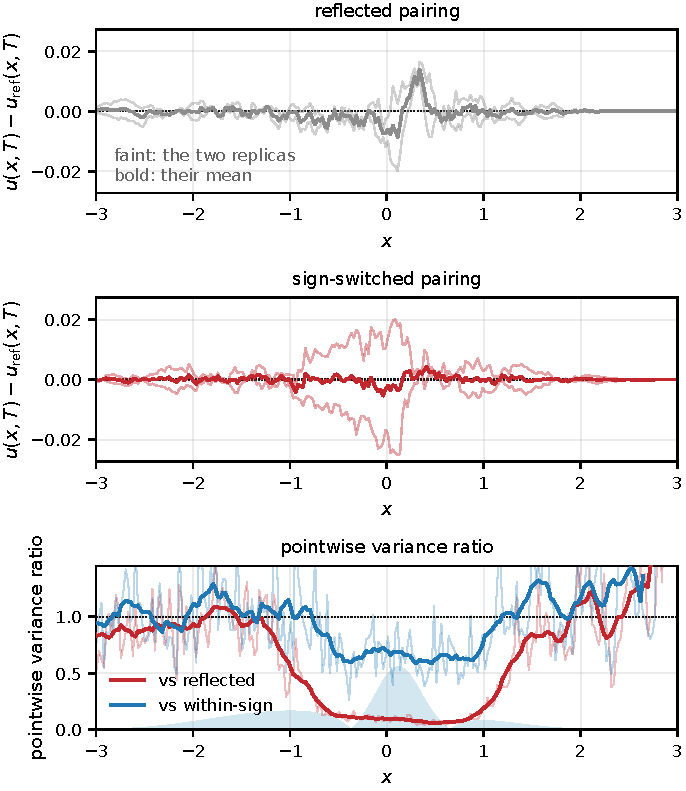
\includegraphics[width=\textwidth]{fig2_fields.pdf}
\caption{Two-pulse Burgers, $N=8192$, $48$ replicates, from the independently
replayed archive. Left and centre: the pointwise error of each replica (faint)
and of their mean (bold) on one replicate. Right: the ratio of pointwise
variance of the sign-switched pair mean to that of the reflected (red) and
within-sign (blue) pair means; thin lines are the raw ratios over $48$
replicates and thick lines a $13$-point running mean. The shaded profile is
$|\partial_x u_{\mathrm{ref}}|$, scaled to the panel.}
\label{fig:fields}
\end{figure}

\paragraph{Cost.} A pair costs $1.93$ times a single trajectory at $N=8192$
($0.1950$\,s against $0.1009$\,s, serial, from experiment A). In a separate
interleaved timing batch, among the three pairings, at
$N=8192$ one replicate costs $0.1941$\,s (reflected), $0.1995$\,s
(sign-switched) and $0.2117$\,s (within-sign): the switch costs $1.028$ times
reflected pairing and $0.943$ times within-sign pairing, and at $N=2048$ the
corresponding figures are $1.040$ and $0.908$. Combining the measured cost with
Table~\ref{tab:headline} gives a variance$\,\times\,$cost ratio of $0.697$
against within-sign pairing. \textbf{These are implementation results.} In these
experiments the sign classes always have equal counts in both replicas, so the
handling of unequal counts cannot be what makes within-sign pairing slower here;
partitioning and gathering are the plausible causes, but we did not profile, and
we therefore do not claim an intrinsic cost advantage over all within-sign
implementations. Timings are serial and single-machine.

\paragraph{Against variance reduction that does not change the coupling.}
Table~\ref{tab:controls} compares the couplings with four alternatives applied
to the same solver: conditional averaging of the final diffusion stage (RB),
which replaces the terminal field by its exact conditional expectation; a known-mean heat control (CVH); and a known-mean control built from a
frozen initial velocity attached to each particle identity (CVF), each with unit
coefficient and with a coefficient fitted on a disjoint training batch. All arms
share seed streams, so the intervals are paired.
For a pre-final configuration $(a_i,m_i)$, this conditional field is
\[
 u_-+\sum_i m_i\Phi((x-a_i)/\sigma),
\]
averaged over the two replicas. It integrates the indicator rather than setting
the displacement to zero. The heat and frozen-velocity controls use each
particle identity's accumulated Brownian displacement $W_i$ and terminal
surrogates $X_i^0+W_i$ and $X_i^0+v_i^0T+W_i$, respectively. Their exact means
are
\[
 \mu_H(x)=u_-+\sum_i m_i\Phi\!\left(\frac{x-X_i^0}{\sqrt{2\nu T}}\right),
 \quad
 \mu_F(x)=u_-+\sum_i m_i\Phi\!\left(\frac{x-X_i^0-v_i^0T}{\sqrt{2\nu T}}\right).
\]
Here $v_i^0$ is the deterministic initial rank velocity, carried by identity in
the surrogate. Predictable sign/permutation transforms preserve the conditional
Gaussian law of each identity's fresh increment, hence its accumulated
increment has law $\mathcal N(0,2\nu T)$. This proves the displayed means for
the discrete initialization. A control estimator is $\bar U-c(\bar H-\mu_H)$
or its frozen-velocity counterpart. The fitted scalar $c$ minimizes integrated
variance on a disjoint training sample by dividing integrated sample covariance
by integrated control variance; it is then held fixed for evaluation.


\begin{table}[htbp]
\centering
\caption{Alternatives on the same solver: integrated variance relative to
reflected pairing, with paired whole-replicate bootstrap intervals, at
$N=1600$, $h=0.005$, $64$ seeds. ``v$\times$c'' multiplies the variance ratio by
the measured per-replicate cost ratio; one-off coefficient training, where
required, is listed separately and is not amortised in v$\times$c. $c^{*}$
denotes a coefficient fitted on a disjoint batch and frozen.}
\label{tab:controls}
\small
\begin{tabular}{llcccc}
\toprule
flux & arm & variance $/$ reflected & v$\times$c & one-off (s) & variance $/$ within-sign\\
\midrule
Burgers & reflected              & 1.0000 & 1.000 & -- & --\\
        & \;+ conditional final stage & 0.8813 $[0.852,0.909]$ & 1.612 & -- & --\\
        & \;+ heat control, $c^{*}$   & 0.8440 $[0.821,0.869]$ & 1.170 & 0.488 & --\\
        & \;+ frozen-velocity control, $c^{*}$ & 0.6724 $[0.617,0.740]$ & 0.923 & 0.466 & --\\
        & within-sign            & 0.2083 $[0.179,0.245]$ & 0.243 & -- & 1\\
        & \textbf{sign-switched} & \textbf{0.1649} $[0.142,0.194]$ & \textbf{0.174} & -- & 0.7916 $[0.762,0.825]$\\
        & \;+ frozen-velocity control, $c^{*}$ & 0.1642 $[0.141,0.194]$ & 0.237 & 0.490 & 0.7886 $[0.758,0.822]$\\
        & \;+ conditional final stage & 0.0804 $[0.069,0.095]$ & 0.151 & -- & 0.3861 $[0.362,0.412]$\\
\midrule
cubic   & reflected              & 1.0000 & 1.000 & -- & --\\
        & \;+ frozen-velocity control, $c^{*}$ & 0.5031 $[0.458,0.552]$ & 0.697 & 0.448 & --\\
        & within-sign            & 0.2263 $[0.196,0.262]$ & 0.268 & -- & 1\\
        & \textbf{sign-switched} & \textbf{0.1739} $[0.151,0.201]$ & \textbf{0.184} & -- & 0.7688 $[0.741,0.797]$\\
        & \;+ heat control, $c^{*}$ & 0.1684 $[0.146,0.194]$ & 0.248 & 0.496 & 0.7442 $[0.716,0.773]$\\
        & \;+ conditional final stage & 0.0818 $[0.070,0.096]$ & 0.158 & -- & 0.3614 $[0.340,0.383]$\\
\bottomrule
\end{tabular}
\end{table}

Three things in Table~\ref{tab:controls} matter. First, the best control-variate
arm built on reflected pairing reaches variance $0.672$ but
variance$\,\times\,$cost $0.923$ on Burgers, before its $0.47$\,s of coefficient
training: the sign switch is more effective than this control addition at the reported cell. Second, once the coupling is switched, a scalar control adds
essentially nothing on Burgers ($0.1649\to0.1642$) and little on the cubic flux
($0.1739\to0.1684$, a resolved but modest $0.968$); this is a statement about
these two controls at these configurations and not a claim that no control can
help. Third, conditional averaging of the final stage is \emph{complementary}
rather than competing: applied on top of the switched coupling it halves the
variance again and gives the best variance$\,\times\,$cost in the table
($0.151$). Its work benefit depends on the cost of evaluating the conditional CDF sum: in
a grid-sensitivity test the additional variance--cost ratio changes from
$0.614$ at $201$ probes to $1.485$ at $1601$ probes. Thus its variance guarantee
does not guarantee lower computational work. We keep the two
separate throughout so that the coupling's contribution is never inflated by
conditioning.

A fourth alternative, a randomised quasi-Monte Carlo adaptation of
\citeauthor{lecot_rims2001}'s idea applied to our transport solver, is included in
the held-out experiment in \S\ref{sec:heldoutA}; it attained the target with
$46$ trajectories against four.

\subsection{Dependence on profile, time, and flux}
\label{sec:qB}

We next vary the initial profile, observation time, and flux to test the scope
of the fixed-setting comparison.

\paragraph{Profiles and times.} Three fixed initial profiles have different sign structures: a
single bump ($2$ regions), the two-pulse profile \eqref{eq:twopulse} ($3$), and
an oscillatory profile $0.45\sin(3x)e^{-x^2/(2\cdot1.1^2)}$ ($13$). Each is
observed at $T=0.25$, $1.0$ and $2.0$ with $N=2048$ and $48$ replicates.
Table~\ref{tab:ladder} and the left panel of Figure~\ref{fig:profiles} give the
result.

\begin{table}[htbp]
\centering
\caption{Integrated variance ratio of sign-switched to within-sign pairing,
$N=2048$, $h=0.005$, $48$ replicates, whole-replicate bootstrap intervals.}
\label{tab:ladder}
\begin{tabular}{lcccc}
\toprule
profile & sign regions & $T=0.25$ & $T=1.0$ & $T=2.0$\\
\midrule
single bump  & 2  & 0.958 $[0.886,1.039]$ & 0.790 $[0.727,0.862]$ & 0.810 $[0.735,0.893]$\\
two-pulse    & 3  & 0.895 $[0.830,0.967]$ & 0.785 $[0.713,0.866]$ & 0.793 $[0.702,0.889]$\\
oscillatory  & 13 & 0.932 $[0.876,0.990]$ & 0.667 $[0.613,0.725]$ & 0.595 $[0.544,0.655]$\\
\bottomrule
\end{tabular}
\end{table}

Eight of the nine cells resolve an advantage. The exception is the single bump
at the earliest time, $0.958$ $[0.886,1.039]$, which is unresolved -- meaning no
resolved advantage at $48$ replicates, not that the benefit disappears. The
advantage is larger at $T=1$ and $T=2$ than at $T=0.25$ in every profile, and
is largest for the oscillatory profile at the two later times. It is
\textbf{not} monotone in time: the single bump moves from $0.790$ to $0.810$ and
the two-pulse profile from $0.785$ to $0.793$ between $T=1$ and $T=2$. The
supported statement is that the advantage is stronger at the later times than at
the earliest time in these examples.

\paragraph{What this does and does not isolate.} The three profiles differ in
amplitude, shape and gradient magnitude as well as in the number of sign
regions, so interleaving is \emph{not} isolated as the cause of the difference
between them. We report the ordering as an observation, not a demonstration.

\begin{table}[htbp]
\centering
\caption{Mean matched-pair separation under rank matching divided by that under
within-sign matching, both rules applied to the \emph{same} paired state so the
history is held fixed; $N=2048$, $24$ replicates, $\pm2$ standard errors. By
Remark~\ref{rem:sorted} every entry is at most $1$ with probability one; what
varies is the size of the gap.}
\label{tab:separation}
\begin{tabular}{lcccc}
\toprule
profile & sign regions & $T=0.25$ & $T=1.0$ & $T=2.0$\\
\midrule
single bump  & 2  & 0.928 $[0.908,0.948]$ & 0.851 $[0.817,0.885]$ & 0.790 $[0.741,0.840]$\\
two-pulse    & 3  & 0.897 $[0.879,0.916]$ & 0.839 $[0.803,0.875]$ & 0.820 $[0.762,0.878]$\\
oscillatory  & 13 & 0.847 $[0.832,0.862]$ & 0.693 $[0.655,0.732]$ & 0.676 $[0.624,0.728]$\\
\bottomrule
\end{tabular}
\end{table}

\begin{figure}[htbp]
\centering
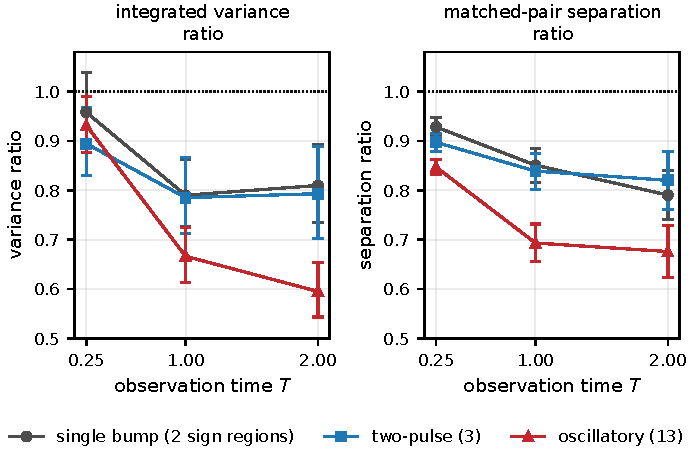
\includegraphics[width=\textwidth]{fig3_profiles.pdf}
\caption{Left: integrated variance ratio of sign-switched to within-sign
pairing across three fixed profiles and three observation times
(Table~\ref{tab:ladder}). Right: the matched-pair separation ratio at a fixed
paired state (Table~\ref{tab:separation}), which cannot exceed $1$ by
Remark~\ref{rem:sorted}; it measures the geometric cost of constraining the
matching to respect sign classes, not the variance mechanism.}
\label{fig:profiles}
\end{figure}

Table~\ref{tab:separation} reports the associated geometry.
Proposition~\ref{prop:finalstage} makes the final-stage gain depend on matched
separation relative to $\sigma$, and the sign-class constraint does cost
geometric slack, most at the oscillatory profile and at later times. But
Remark~\ref{rem:sorted} shows that the direction of this table is fixed in
advance: rank matching is the optimal matching for absolute distance, so the
ratio is at most $1$ whatever the configuration. The table quantifies the size
of the slack; it cannot establish that the slack causes the variance
difference, and the two orderings are not even identical -- the separation ratio
at $T=2$ orders the profiles oscillatory $<$ single bump $<$ two-pulse while the
variance ratio orders them oscillatory $<$ two-pulse $<$ single bump. We
therefore report the association and not a mechanism.

A separate diagnostic lets each matching rule act on its own evolved state.
That comparison mixes geometry with coupling history and is recorded as a
supporting association in the evidence archive; it is not used to infer a
variance mechanism.

\paragraph{Flux.} Replacing $f(u)=u^2/2$ by $f(u)=u^3/3$ changes the character
of the transport: $f'(u)=u^2\ge0$ vanishes at $u=0$ without changing sign, so
there is no left/right propagation, and $f''(u)=2u$ makes the characteristic
speed non-affine. With everything else held fixed at $N=1600$, $h=0.005$ and the
same $64$ seeds, the sign-switched--to--within-sign variance ratio is
$0.7916$ $[0.762,0.825]$ for Burgers and $0.7688$ $[0.741,0.797]$ for the cubic
flux (Table~\ref{tab:controls}). The advantage does not require bidirectional
transport. This comparison does not establish transfer to arbitrary fluxes.

\subsection{Work at selected accuracy targets}
\label{sec:qC}

Variance ratios at fixed settings are not work. We ran two held-out experiments.
In each, a pilot on one seed key supplied plug-in estimates of $b^2$, $V$ and
the per-replicate cost $C$ for every arm; the replicate count of each arm was
then \emph{frozen} at the smallest integer $B$ with
$b^2_{\mathrm{hi}}+V_{\mathrm{hi}}/B\le\mathrm{tol}/\kappa$, using upper
endpoints and a safety factor $\kappa=1.3$; and the frozen plans were evaluated
on an unused seed key with $32$ independent blocks. At each cell the paired and single arms use the
switched pilot estimate of the shared bias; the RQMC arm uses its own estimate.
The experiments differ in
their target, their $N$, and their arms, and we keep them separate rather than
pooling them: the first was designed before within-sign pairing was added as a
comparator and does not contain it.

\subsubsection{Experiment A: against an unpaired ensemble, reflected pairing,
and a randomised quasi-Monte Carlo adaptation}
\label{sec:heldoutA}

Target $7\times10^{-6}$ expected integrated squared field error, $N=8192$,
pilot key $1601$, evaluation key $1702$. The target was chosen from the pilot,
so it is a pilot-informed target with an independent evaluation batch.

The quasi-Monte Carlo arm is an adaptation of \citeauthor{lecot_rims2001}'s
rank-based diffusion to our transport solver, not a reproduction of his method.
One \texttt{scipy.stats.qmc.Sobol} engine with $d=2$ and $30$ bits is created per
replicate and scrambled once; successive time steps consume successive blocks of
$N$ points, as in his equation~(45). SciPy's \texttt{scramble=True} is a
left-matrix scramble combined with a digital random shift, not fully nested Owen
scrambling \citep{owen1998,virtanen2020}. The first coordinate assigns a rank by
$\lfloor N p_1\rfloor$ and the second supplies the increment
$\sigma\Phi^{-1}(p_2)$, with $p_2$ clipped to $[2^{-53},1-2^{-53}]$ and the clip
count recorded. $N$ must be a power of two. We do not claim this adaptation
preserves the interacting discrete law; its total error is measured
independently, including its own bias. The rank-bijection assertion is checked outside the timed path.

\begin{table}[htbp]
\centering
\caption{Held-out experiment A. Frozen plans, unused evaluation key, $32$
blocks, $N=8192$, target $7\times10^{-6}$. ``Trajectories'' counts solver runs,
which is $2B$ for a paired arm and $B$ otherwise. The upper bound is a
Bonferroni-corrected $95\%$ $t$ bound across the four arms
($t_{31,\,1-0.05/8}=2.652$); every arm's bound lies below the target.}
\label{tab:heldoutA}
\begin{tabular}{lccccc}
\toprule
arm & $B$ & trajectories & attained error & simultaneous upper bound & measured work (s)\\
\midrule
unpaired ensemble        & 65 & 65 & $5.347\times10^{-6}$ & $6.743\times10^{-6}$ & 6.658\\
reflected pairing        & 17 & 34 & $5.031\times10^{-6}$ & $6.362\times10^{-6}$ & 3.340\\
RQMC adaptation          & 46 & 46 & $4.024\times10^{-6}$ & $4.873\times10^{-6}$ & 6.848\\
\textbf{sign-switched pairing} & \textbf{2} & \textbf{4} & $5.100\times10^{-6}$ & $5.611\times10^{-6}$ & \textbf{0.407}\\
\bottomrule
\end{tabular}
\end{table}

\subsubsection{Experiment B: against within-sign pairing}
\label{sec:heldoutB}

Target $2.5\times10^{-5}$, $N=2048$, pilot key $2310$, evaluation key $2320$,
$32$ blocks, tuning cost $4.05$\,s reported separately. This experiment uses the
standard two-pulse configuration rather than the oscillatory profile that
favours the construction.

\begin{table}[htbp]
\centering
\caption{Held-out experiment B. Frozen plans, unused evaluation key, $32$
blocks, $N=2048$, target $2.5\times10^{-5}$, Bonferroni bound across three arms
($t_{31,\,1-0.05/6}=2.531$). Work is end-to-end with interleaved arm order.}
\label{tab:heldoutB}
\begin{tabular}{lccccc}
\toprule
arm & $B$ & trajectories & attained error & simultaneous upper bound & measured work (s)\\
\midrule
reflected pairing        & 18 & 36 & $1.404\times10^{-5}$ & $1.830\times10^{-5}$ & 0.615\\
within-sign pairing      &  3 &  6 & $1.769\times10^{-5}$ & $1.936\times10^{-5}$ & 0.119\\
\textbf{sign-switched pairing} & \textbf{2} & \textbf{4} & $1.976\times10^{-5}$ & $2.203\times10^{-5}$ & \textbf{0.0715}\\
\bottomrule
\end{tabular}
\end{table}

All three arms attain the target, pointwise and simultaneously. The measured
work ratio is $0.599$ against within-sign pairing and $0.116$ against reflected
pairing. \textbf{Three qualifications belong with those numbers.} The arms did
not land at equal attained error -- reflected pairing overshoots the target most
and the switched arm sits closest to it -- so this is selected-plan attainment,
not equal-error performance. At $B=2$ against $B=3$ the integer granularity
carries much of the ratio: $\tfrac23$ times the cost ratio $0.908$ is $0.605$,
close to the measured $0.599$, so the experiment mainly confirms that the
switched arm needs one fewer replicate here. And the plans were selected from a
pilot rather than optimised.

Both experiments are reported in Figure~\ref{fig:heldout}. For experiment B,
the original evaluation collected errors with sequential arm timing. Reported
work comes from a separate interleaved timing of the same frozen plans; reported
errors remain those of the original held-out batch.

\begin{figure}[htbp]
\centering
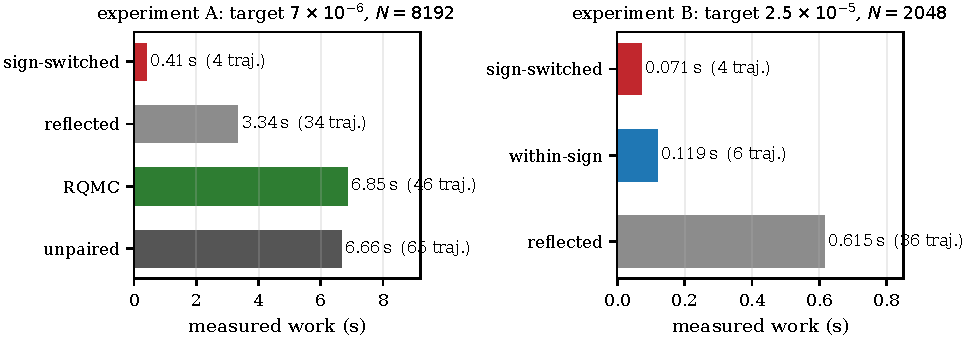
\includegraphics[width=\textwidth]{fig4_heldout.pdf}
\caption{Measured work to attain a common expected-error target in the two
held-out experiments, which have different targets, different $N$ and different
arms and are not to be pooled. Left: experiment A
(Table~\ref{tab:heldoutA}). Right: experiment B (Table~\ref{tab:heldoutB}).}
\label{fig:heldout}
\end{figure}

\subsection{Observable dependence and the bias-dominated regime}
\label{sec:qD}

\subsubsection{The benefit is not uniform over the domain}

At $N=8192$ with $48$ replicates on a separate seed key, the variance ratio of
sign-switched to reflected pairing at four probe locations is
$0.636$ $[0.357,1.135]$ at the left flank $x=-2.0$,
$0.143$ $[0.080,0.255]$ at the left pulse $x=-0.7$,
$0.093$ $[0.052,0.166]$ at the steepest core $x=+0.1$, and
$0.735$ $[0.412,1.311]$ at the right flank $x=+1.5$
($F(47,47)$ intervals). The two flank comparisons are unresolved. A reader whose
quantity of interest lives where the field is flat should not expect the
integrated figure.

\subsubsection{For a nonlinear functional, a variance ratio is not an accuracy
ratio}

Let $Q$ be a nonlinear functional of the field. The two natural estimators,
$Q(\bar U)$ and $\tfrac12\bigl(Q(U^{(A)})+Q(U^{(B)})\bigr)$, have different
expectations. By Proposition~\ref{prop:law} the second has exactly the
expectation of $Q$ applied to a single uncoupled run, so its bias is the
single-run bias whatever the coupling; the first has no such guarantee. We
therefore report the \emph{empirical} mean squared error against the reference,
\begin{equation}
  \widehat{\mathrm{MSE}}
  =\frac1n\sum_{r=1}^{n}\bigl(Q_r-Q_{\mathrm{ref}}\bigr)^2
  =\widehat{\mathrm{bias}}^2+\frac{n-1}{n}\,s^2 ,
  \label{eq:empmse}
\end{equation}
and not the plug-in $\widehat{\mathrm{bias}}^2+s^2$, which exceeds
\eqref{eq:empmse} by $s^2/n$ (here $0.7\%$--$2.0\%$). Table~\ref{tab:nonlinear}
uses \eqref{eq:empmse} throughout. Two functionals are reported, and both are
rule-dependent, so the rules are stated: $\max|\partial_x u|$ uses central
differences of the reconstructed field on the output grid and is
grid-dependent; the level crossing is the first downward crossing of $u=0.25$ to
the right of the global maximum, by linear interpolation, with replicates
lacking such a crossing recorded as censored (none occurred in any cell).

\begin{table}[htbp]
\centering
\caption{Nonlinear observables at $N=8192$, $48$ replicates, against the
spectral reference, from the independently replayed archive. Ratios are of the
empirical mean squared error \eqref{eq:empmse}, with whole-replicate bootstrap
intervals; the last column is the squared-bias share of the sign-switched arm's
empirical MSE. An interval containing $1$ is unresolved.}
\label{tab:nonlinear}
\small
\begin{tabular}{llccc}
\toprule
functional & estimator & switched $/$ reflected & switched $/$ within-sign & bias$^2$ share\\
\midrule
$\max|\partial_x u|$ & $Q$ of the mean      & 0.416 $[0.244,0.702]$ & 0.602 $[0.359,0.984]$ & 0.56\\
                     & mean of $Q$          & 0.832 $[0.603,1.139]$ & 1.058 $[0.803,1.394]$ & 0.87\\
level $x(u=0.25)$    & $Q$ of the mean      & 0.129 $[0.070,0.247]$ & 0.855 $[0.497,1.419]$ & 0.19\\
                     & mean of $Q$          & 0.090 $[0.053,0.158]$ & 0.847 $[0.497,1.486]$ & 0.30\\
\bottomrule
\end{tabular}
\end{table}

Table~\ref{tab:nonlinear} contains the clearest applicability boundary in the
paper. For the level crossing the switched coupling reduces total error by
roughly an order of magnitude against reflected pairing under either estimator.
For the peak gradient it does not: with the mean-of-$Q$ estimator the ratio
against reflected pairing is $0.832$ $[0.603,1.139]$ and against within-sign
pairing $1.058$ $[0.803,1.394]$, both unresolved. The plug-in squared-bias share is $87\%$ for that estimator;
it is itself estimated, and Corollary~\ref{cor:bias} establishes sharing of the
population bias across the couplings, not exact equality of finite-sample estimates. A variance reduction can only reduce the sampling component of this error. The corresponding variance ratios are $0.410$ ($Q$ of the mean)
and $0.686$ (mean of $Q$) against reflected pairing -- a factor of $2.4$ and
$1.5$, not ten.

\subsubsection{The bias-dominated regime}

The same arithmetic applies to the field itself. Since the couplings share
$b^2$, \eqref{eq:decomposition} gives
\begin{equation}
  \frac{\mathcal E_{\swi}(B)}{\mathcal E_{\refl}(B)}
  =\frac{b^2+V_{\swi}/B}{b^2+V_{\refl}/B}\;\longrightarrow\;1
  \qquad\text{as } B\to\infty ,
  \label{eq:crossover}
\end{equation}
when $b^2>0$. If $b^2=0$, the ratio instead remains $V_{\swi}/V_{\refl}$.
Thus the crossover concerns nonzero baseline bias at fixed $N$ and $h$. The
scale on which it fades is $B^{\star}=V/b^2$, at which the sampling and
discretisation contributions are equal. At three archived cells of the two-pulse
problem $B^{\star}$ for the switched arm is $10.3$ ($N=6400$, $h=0.0025$),
$4.5$ ($N=6400$, $h=0.005$) and $35.3$ ($N=1600$, $h=0.0025$).
Figure~\ref{fig:bias} uses equal continuous work instead of equal pair counts:
\begin{equation}
 \frac{b^2+V_{\swi}C_{\swi}/W}{b^2+V_{\refl}C_{\refl}/W}.
 \label{eq:equalwork}
\end{equation}
This is a plug-in model, excluding integer allocation and timing uncertainty.
The crossover marks equal sampling and bias contributions in the switched arm;
it is not a cutoff for improvement.

\begin{figure}[htbp]
\centering
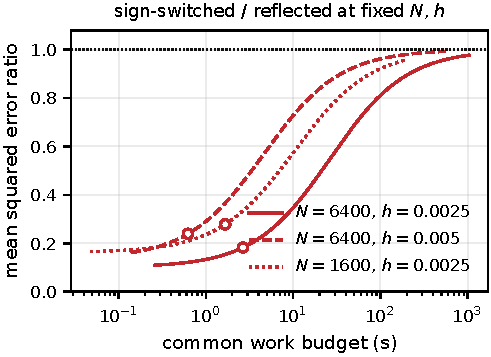
\includegraphics[width=0.52\textwidth]{fig5_bias.pdf}
\caption{Model mean squared error ratio \eqref{eq:equalwork} at equal work, at three
archived $(N,h)$ cells of the two-pulse problem with $64$ paired seeds. The
shared squared bias $b^2$ is the same estimate in numerator and denominator,
as Corollary~\ref{cor:bias} requires. Circles mark $W=C_{\swi}V_{\swi}/b^2$. Three
cells indicate a direction; they do not establish a rate, and they do not
separate the effects of $N$ and $h$.}
\label{fig:bias}
\end{figure}

The practical reading is the one a reader can act on: the coupling buys
accuracy when the ensemble is small enough that sampling error still matters,
which is exactly the regime in which one is paying for solver trajectories. When
the discretisation error dominates, refine $N$ or $h$; no coupling will help.

\subsection{Signed-structure controls}
\label{sec:structure}

Table~\ref{tab:structure} maps the effect against the signed structure of the
initial data at a production cell. The rows are informative in different ways
and must not be read alike.

\begin{table}[htbp]
\centering
\caption{Integrated variance ratio of sign-switched to reflected pairing by
signed structure, $N=2048$, $h=0.005$, $T=1$, $48$ replicates, whole-replicate
bootstrap intervals. The two arms of each cell were run on \emph{different} seed
streams, so these are ratios of independent estimates; the one-sign row is
therefore an estimate of a quantity that Corollary~\ref{cor:onesign} makes
exactly $1$, and its departure from $1$ is sampling noise. Exact identity is
established separately, by a matched-seed full-state comparison.}
\label{tab:structure}
\begin{tabular}{llcc}
\toprule
structure & dynamics & variance ratio & reading\\
\midrule
interleaved (alternating signs) & heat    & 0.049 $[0.040,0.061]$ & resolved help\\
                                & Burgers & 0.063 $[0.052,0.077]$ & resolved help\\
merging blocks                  & heat    & 0.476 $[0.421,0.545]$ & resolved help\\
                                & Burgers & 0.481 $[0.426,0.544]$ & resolved help\\
separated blocks                & heat    & 0.994 $[0.917,1.076]$ & unresolved\\
                                & Burgers & 1.013 $[0.930,1.101]$ & unresolved\\
one sign                        & heat    & 0.987 $[0.902,1.078]$ & exactly 1 by Cor.~\ref{cor:onesign}\\
                                & Burgers & 0.967 $[0.822,1.174]$ & exactly 1 by Cor.~\ref{cor:onesign}\\
\bottomrule
\end{tabular}
\end{table}

\paragraph{The interleaved configuration is a mechanism test, not a refinement
study.} Its alternating masses $\pm1/N$ on a fixed support give a reconstructed
field whose amplitude falls like $1/N$: it is $2.5\times10^{-3}$ at $N=400$
and $1.2\times10^{-4}$ at $N=8192$, while the total absolute mass stays at $1$.
Increasing $N$ therefore changes the represented field, not merely its
resolution, and its ratios must not be read as convergence under refinement. The
merging and separated configurations hold the amplitude at $0.5$ and \emph{are}
refinements of one fixed profile.

\paragraph{Separated blocks.} The unresolved rows are consistent with the
divergence analysis of \S\ref{sec:theory}: the two couplings agree on about
$71\%$ of seeds and, when they do diverge, do so at a median step of $187$ out
of $200$, leaving little history over which a difference can accumulate. This is
a statement about this configuration at this $N$, $h$, $\nu$ and horizon.

\paragraph{One sign.} The two couplings are the same algorithm
(Corollary~\ref{cor:onesign}); the row is a consistency check on the estimator,
not evidence. The exact statement comes from a matched-seed comparison of the
complete state -- positions, masses and carried velocities -- which gives a
maximum absolute difference of exactly $0$ over $200$ seeds for each dynamics.

% Exploratory predictor retained in the research archive, not in this manuscript.

\section{Discussion}
\label{sec:discussion}

The experiments distinguish two gains. Respecting mass signs through
within-sign matching accounts for most of the improvement over reflected
rank pairing. Retaining spatial-rank matching and switching the increment
orientation gives an additional reduction, resolved in the principal field
comparison and in the tested later-time profiles. The held-out experiment
including within-sign pairing demonstrates a practical consequence for one
selected accuracy target. Its coarse integer allocations and unequal attained
errors limit interpretation as an optimized efficiency comparison.

The exact final-stage identity identifies how opposite signs, mass magnitudes,
and separations affect conditional covariance. It does not characterize
variance accumulated through the nonlinear histories. The separation diagnostic
quantifies the geometric restriction imposed by within-sign matching; the
optimality of sorted matching for absolute distance does not establish
optimality for field variance. The profile comparison also changes amplitudes
and gradients, so its ordering does not isolate sign-region count as a cause.

The practical benefit depends on the requested output and the balance between
sampling error and baseline bias. One-sign data make the switched and reflected
rules identical, while mixed-sign data can also produce little resolved gain.
Nonlinear functions of the averaged field have coupling-dependent expectations.
Consequently the appropriate comparison is total error for the chosen output,
with the number of trajectories and execution cost reported separately.

The scope is scalar, one-dimensional mean transport with constant particle
masses. The proof of marginal preservation accommodates broader predictable
couplings, but neither a multidimensional matching rule nor a coupling for a
sampled-velocity solver is evaluated here. All timings are serial. Parallel
communication costs, finer work-to-target comparisons, and sufficient
conditions for nonlinear terminal variance reduction remain open.

\section{Conclusion}
\label{sec:conclusion}

Sign-aware antithetic coupling combines spatial-rank matching with an increment
orientation determined by the matched gradient masses. It preserves each
replica's discrete law and reduces conditional integrated variance relative to
reflection when applied at the final diffusion stage. The full-history benefit
is assessed numerically. In the principal two-pulse experiment, integrated
variance is $0.739$ times that of within-sign pairing, with approximate $95\%$
interval $[0.682,0.801]$, and integrated MSE is $0.819$ times as large. In a
separate held-out comparison, four trajectories attain the selected target
against six for within-sign pairing, at approximately $0.60$ of its execution
work. Fixed-profile and cubic-flux comparisons extend the empirical evidence,
while one-sign controls, weak-benefit cases, and bias-dominated observables
define its limits. The resulting estimator provides a simple additional option
for users of signed gradient-particle solvers, with guarantees restricted to the
properties proved here.

\section*{Data and code availability}

The manuscript source, figure-generation scripts, numerical evidence, and
reproduction instructions are distributed with the accompanying repository at
\url{https://github.com/stephen122204/rb-gbmc-viscous-burgers}.
The evidence map records source files and statistical conventions for each
reported result. Historical exploratory outputs are distinguished from the
curated evidence used by this manuscript.

\bibliographystyle{unsrtnat}
\bibliography{references-coupling}

\appendix
% =====================================================================
\section{Proofs}
\label{app:proofs}

\subsection{Proposition~\ref{prop:law}}

Write $\Xi^A_k=(X^A_k,m^A_k,v^A_k)$ for replica $A$'s state after stage $k$ and
$\Fil_k$ for the $\sigma$-field generated by the joint history up to and
including the sort and velocity update of stage $k$. The transport, sort and
velocity update of Algorithm~\ref{alg:single} are deterministic functions of
$\Xi^A_{k-1}$ alone. It therefore suffices to show that, conditionally on
$\Fil_k$, the vector of increments applied to replica $A$ is
$\mathcal N(0,\sigma^2 I_N)$, and likewise for $B$.

For $A$ this is immediate: $Z^{(k)}\sim\mathcal N(0,I_N)$ is drawn independently
of $\Fil_k$. For $B$, the applied increment is
$\sigma\varepsilon_{k,j}Z^{(k)}_{\pi_k(j)}$ with $(\pi_k,\varepsilon_k)$
$\Fil_k$-measurable. Conditionally on $\Fil_k$ the pair
$(\pi_k,\varepsilon_k)$ is a fixed bijection and a fixed sign vector, while
$Z^{(k)}$ remains $\mathcal N(0,I_N)$; a permutation of the coordinates of an
i.i.d.\ standard Gaussian vector is i.i.d.\ standard Gaussian, and multiplying
coordinate $j$ by a constant of modulus one leaves its law $\mathcal N(0,1)$ and
preserves independence across $j$ because the permutation is injective. Hence
replica $B$'s conditional increment law is $\mathcal N(0,\sigma^2I_N)$, the same
as an uncoupled run's. Induction over $k=1,\dots,K$ gives equality of the laws
of the complete state trajectories. Only the joint law of $(\Xi^A,\Xi^B)$ is
changed, since the increments of the two replicas are now dependent. \qed

Each hypothesis is used: freshness and independence of $Z^{(k)}$ from $\Fil_k$
for the conditional law; bijectivity of $\pi_k$ for independence across
coordinates; unit modulus for the variance; measurability with respect to
$\Fil_k$ so that the multipliers are not chosen after seeing the draw;
exclusion of zero masses so that \eqref{eq:switch} has modulus one; and
retention of the particle--velocity association until transport so that $\Xi$
is the complete state.

\subsection{Lemma~\ref{lem:wholeline}}

Fix $c\in\R$ and set $h_a(x)=\ind\{x\ge a\}-\ind\{x\ge c\}$, which is compactly
supported with $\int h_a h_b\,\mathrm dx=\tfrac12(|a-c|+|b-c|-|a-b|)$ by direct
computation. Since $\sum_i m^A_i=\sum_j m^B_j=0$ we may write
$D_A=\sum_i m^A_i h_{X^A_i}$ and $D_B=\sum_j m^B_j h_{X^B_j}$, both compactly
supported. Then
\[
  \int D_AD_B
  =\sum_{i,j}m^A_im^B_j\,\tfrac12\bigl(|X^A_i-c|+|X^B_j-c|-|X^A_i-X^B_j|\bigr),
\]
and the first two groups of terms vanish because
$\sum_j m^B_j=0$ and $\sum_i m^A_i=0$ respectively. \qed

\subsection{Proposition~\ref{prop:finalstage}}

Condition on the pre-final state. Write $D_\bullet$ as in
Lemma~\ref{lem:wholeline} for the terminal configurations, so that
$\bar U=u_-+\tfrac12(D_A+D_B)$ and
\[
  V_\bullet=\int\Var\bar U
  =\tfrac14\Bigl(\int\Var D_A+\int\Var D_B+2\int\mathrm{Cov}(D_A,D_B)\Bigr).
\]
By Proposition~\ref{prop:law} the first two integrals do not depend on the
coupling. For the third, Lemma~\ref{lem:wholeline} applied to
$\E\!\int\! D_AD_B$ and, separately, to $\int\E D_A\,\E D_B$ -- the latter by
introducing an independent copy $Z'$ of the noise and using
$\E D_A(x)=\E_{Z}[\,\cdot\,]$ -- gives
\[
  \int\mathrm{Cov}(D_A,D_B)
  =-\tfrac12\sum_{i,j}m^A_im^B_j
     \Bigl[\E\bigl|X^A_i-X^B_j\bigr|-g_{\sigma\sqrt2}(a_i-b_j)\Bigr].
\]
For $i\ne j$ the increments $Z_i$ and $\varepsilon_jZ_j$ are independent with
variance $\sigma^2$ each under \refl{} and \swi{}, so
$X^A_i-X^B_j=(a_i-b_j)+\sigma\sqrt2\,\mathcal N(0,1)$ in law and the bracket
vanishes. Only the diagonal survives. There, under \refl{},
$X^A_i-X^B_i=d_i+2\sigma Z_i$ and the first term is $g_{2\sigma}(d_i)$; under
\swi{} it is $g_{2\sigma}(d_i)$ when $m^A_im^B_i>0$ and, when
$m^A_im^B_i<0$, the two increments cancel exactly and the first term is
$|d_i|$. Subtracting,
\[
  \int\mathrm{Cov}_{\refl}-\int\mathrm{Cov}_{\swi}
  =-\tfrac12\!\!\sum_{m^A_im^B_i<0}\!\! m^A_im^B_i\bigl[g_{2\sigma}(d_i)-|d_i|\bigr]
  =\tfrac12\!\!\sum_{m^A_im^B_i<0}\!\!\bigl|m^A_im^B_i\bigr|
     \bigl[g_{2\sigma}(d_i)-|d_i|\bigr],
\]
and multiplying the covariance difference by $1/2$ gives \eqref{eq:finalstage}.
Non-negativity is $g_s(d)=\E|d+sZ|\ge|\E(d+sZ)|=|d|$. \qed

% =====================================================================
\section{A two-particle monotonicity counterexample}
\label{app:counterexample}
Take $u_-=0$, $m=(1/2,-1/2)$, $h=0.005$, $\nu=10^{-10}$, and two steps.
The initial positions are $(p,0)$, with $p_L=-0.00275$ or
$p_R=-0.00225$. Both initial carried velocities are $(1/2,0)$.
Without diffusion, the first transport puts the positive particle at
$-0.00025$ in state $L$ and $+0.00025$ in state $R$. Re-sorting therefore
leaves the velocities $(1/2,0)$ in $L$ but assigns $(-1/2,0)$ to the
negative and positive particles, respectively, in $R$. After the second
transport, the particle positions in identity order are
\[
 L:(0.00225,0),\qquad R:(0.00025,-0.0025).
\]
At the probe $x_*=0.00125$, the reconstructed fields are $-1/2$ and $0$.

Now restore the Gaussian displacements with $\sigma=10^{-6}$. On the event
that each of the four displacements of a trajectory has modulus at most
$\delta=10^{-4}$, neither its second transport ordering nor its terminal
probe classification changes: the relevant ordering gap is $0.00025>2\delta$
and the smallest probe margin is $0.001>2\delta$. Hence the same field values
hold on this event. For either initial state the exceptional probability is
at most $\epsilon=8\Phi(-100)<\exp(-5003)$. Since every field value is in
$[-1/2,1/2]$,
\[
 \E U_R(x_*,2h)-\E U_L(x_*,2h)\ge\tfrac12-\tfrac32\epsilon>0.
\]
The initial movement of a positive mass to the right thus increases the
expected terminal field. This proves the claim in Remark~\ref{rem:mono}
without inferring an expectation from a finite set of simulation seeds.

\section{Test problems, initialisation and reference solutions}
\label{app:setup}

\paragraph{Initialisation.} For the smooth profiles with $u_+=u_-$, let $\mathrm{TV}=\int|u_0'|$. We place
$N/2$ particles at the deterministic midpoint quantiles
$r_k=(k-\tfrac12)/(N/2)$, $k=1,\dots,N/2$, of the normalised positive part of
$u_0'$ and $N/2$ at those of the negative part, assigning
$m_i=\pm\mathrm{TV}/N$. This gives equal counts and equal absolute mass in each
sign class and makes $\sum_i m_i=u_+-u_-$; it is deterministic, so the initial
state is common to both replicas and to every arm.

\paragraph{Profiles.} The two-pulse profile is \eqref{eq:twopulse}. The
single-bump profile is $0.8\,e^{-(x+0.2)^2/(2\cdot0.45^2)}$ and the oscillatory
profile is $0.45\sin(3x)\,e^{-x^2/(2\cdot1.1^2)}$; the number of sign regions of
$u_0'$ quoted for each is computed from a $40\,001$-point evaluation with a
relative magnitude threshold of $10^{-6}$, giving $2$, $3$ and $13$. The four
signed-structure configurations of \S\ref{sec:structure} place $N$ particles of
equal magnitude $1/N$ as follows: \emph{interleaved}, alternating signs on
$[-0.25,0.25]$; \emph{separated}, a positive block on $[-2.0,-1.4]$ and a
negative block on $[1.4,2.0]$; \emph{merging}, blocks on $[-0.9,-0.5]$ and
$[0.5,0.9]$; \emph{one sign}, all masses $-2/N$ on $[-1,1]$.

\paragraph{References.} For $f(u)=u^2/2$ and $f(u)=u^3/3$ the reference is a
Fourier pseudospectral solution on $[-16,16]$ with $M=2048$ modes,
$\tfrac23$-rule dealiasing and integrating-factor RK4 at $\mathrm dt=10^{-4}$.
For Burgers it agrees with a stabilised whole-line Cole--Hopf evaluation
\citep{hopf1950,cole1951} -- the potential $F(y)=\int_0^yu_0$ being analytic for
Gaussian pulses -- to $5.57\times10^{-14}$ in the maximum norm on the output
grid; for the cubic flux, halving $\mathrm dt$ and doubling $M$ moves the
solution by $1.6\times10^{-13}$. These are correctness instruments. They are
never used as cost comparators and never enter the fitting of any control
coefficient.

% =====================================================================
\section{Uncertainty methodology and its calibration}
\label{app:uncertainty}

The two interval procedures used for scalar observables are a whole-replicate
percentile bootstrap and $F(n-1,n-1)$. The second assumes independent normal
replicates, which we do not assert, so we calibrated both.

Per-replicate values of four observables were taken from the archived $N=8192$
fields, \emph{separately} for the reflected and sign-switched arms, and each
sample was centred and scaled by its own standard deviation to give two
empirical shapes. A synthetic numerator arm resamples the sign-switched shape,
scaled to impose a known variance ratio $r$; the denominator arm resamples the
reflected shape. Nominal-$95\%$ intervals are then formed by each procedure and
coverage counted over $M=1500$ synthetic datasets, with $n=48$ per arm and $400$
bootstrap resamples per interval. Table~\ref{tab:calibration} reports the
two-shape design together with the common-shape design of an earlier
calibration, which used one standardised sample for both arms and therefore
could not speak to the case of interest.

\begin{table}[htbp]
\centering
\caption{Coverage of nominal-$95\%$ variance-ratio intervals, $M=1500$
synthetic datasets per cell, binomial standard error $\le0.007$. ``Two-shape''
resamples the sign-switched and reflected empirical shapes separately;
``common-shape'' reproduces the earlier design in which both arms came from one
standardised sample.}
\label{tab:calibration}
\small
\begin{tabular}{lcccccc}
\toprule
& \multicolumn{2}{c}{two-shape, $r=0.15$} & \multicolumn{2}{c}{two-shape, $r=0.75$}
& \multicolumn{2}{c}{common-shape, $r=0.75$}\\
\cmidrule(lr){2-3}\cmidrule(lr){4-5}\cmidrule(lr){6-7}
observable & bootstrap & $F$ & bootstrap & $F$ & bootstrap & $F$\\
\midrule
station $x=+0.1$    & 0.921 & 0.958 & 0.933 & 0.967 & 0.945 & 0.977\\
station $x=-2.0$    & 0.950 & 0.982 & 0.946 & 0.973 & 0.942 & 0.977\\
$\max|\partial_xu|$ & 0.941 & 0.965 & 0.931 & 0.960 & 0.947 & 0.954\\
level $x(u=0.25)$   & 0.933 & 0.959 & 0.928 & 0.949 & 0.935 & 0.963\\
\bottomrule
\end{tabular}
\end{table}

Under the two-shape design, estimated $F$ coverage is $0.949$--$0.982$
and percentile-bootstrap coverage is $0.921$--$0.950$, with simulation uncertainty
as stated in the table. We therefore report $F$ intervals for station and
level-crossing variance ratios and bootstrap intervals for integrated,
and mean-squared-error ratios. The calibration concerns scalar variance ratios;
it does not establish coverage for integrated-field or MSE intervals. Those
bootstrap intervals are approximate, particularly at these sample sizes. This describes performance under \emph{these} empirical
distributions at \emph{this} configuration; it is not a guarantee for other
problems, and a non-significant normality test records failure to reject, not
normality.

% =====================================================================
\section{Evidence provenance}
\label{app:provenance}

Table~\ref{tab:provenance} maps every table and figure to the archived output
that produced it. Paths are relative to the study repository's
\texttt{output/} directory unless stated otherwise; each directory name
carries a date suffix (\texttt{\_2026\_09\_09} or \texttt{\_2026\_09\_10})
which is omitted here for width. The file
\texttt{analysis/numbers.json} contains each quantity together with the archive
it was read from.

\begin{table}[htbp]
\centering
\caption{Provenance of reported results.}
\label{tab:provenance}
\small
\renewcommand{\arraystretch}{1.15}
\begin{tabular}{@{}>{\raggedright\arraybackslash}p{3.0cm}>{\raggedright\arraybackslash}p{3.3cm}>{\raggedright\arraybackslash}p{7.2cm}@{}}
\toprule
item & what it answers & archive\\
\midrule
Table~\ref{tab:headline}, Fig.~\ref{fig:fields}
  & headline field comparison
  & independent replay of \path{round22_corrections};
    \path{replayed_fields.npz}, \path{replay_audit.json}\\
cost figures, \S\ref{sec:qA}
  & what the coupling costs
  & \path{round22_corrections/costs.json};
    \path{round17_compare/compare.json} (pair versus single)\\
Table~\ref{tab:controls}
  & against controls and a second flux
  & \path{round09_costs_control/fields.npz},
    \path{.../rows.csv}\\
Table~\ref{tab:ladder}, Fig.~\ref{fig:profiles} (left)
  & profiles and times
  & \path{round23_mechanism/mechanism.json}\\
Table~\ref{tab:separation}, Fig.~\ref{fig:profiles} (right)
  & matched-pair geometry
  & \path{round24_separation/separation.json}
    (\path{matched_state} rows; the \path{own_history} rows are the
    association-only variant, one of nine cells containing $1$)\\
Table~\ref{tab:heldoutA}, Fig.~\ref{fig:heldout} (left)
  & held-out work, experiment A
  & \path{round17_compare/compare.json}\\
Table~\ref{tab:heldoutB}, Fig.~\ref{fig:heldout} (right)
  & held-out work, experiment B
  & \path{round23_mechanism/worktarget.json};
    interleaved timings from
    \path{round24_separation/timing_check.json}\\
station ratios, \S\ref{sec:qD}
  & where the benefit sits
  & \path{round18_observable/observable.json},
    \path{.../f_intervals.json}\\
Table~\ref{tab:nonlinear}
  & nonlinear observables
  & replayed archive as above; empirical MSE by \eqref{eq:empmse}\\
Fig.~\ref{fig:bias}
  & bias-dominated regime
  & \path{round07_joint_cell/joint_cell.json}\\
Table~\ref{tab:structure}
  & signed-structure map
  & \path{round21_applicability/applicability.json}\\
Prop.~\ref{prop:finalstage} check and share
  & is the identity right, and how much does it explain
  & \path{round25_finalstage/finalstage.json};
    aggregates from \path{round06_finalstep/finalstep.json}\\
Cor.~\ref{cor:onesign}, divergence fractions
  & when are the couplings identical
  & \path{round25_divergence/divergence.json} ($200$ seeds);
    \path{round22_corrections/corrections.json} ($40$ seeds)\\
Prop.~\ref{prop:law} witness
  & does a replica match production
  & \path{round14_audit/audit.json};
    \path{single_vs_production} maximum absolute differences
    $0$ in position, mass and field\\
Rem.~\ref{rem:mono}
  & why there is no unconditional guarantee
  & \path{round07_counterexample/counterexample.json}\\
Table~\ref{tab:calibration}
  & are the intervals trustworthy
  & \path{round25_calibration/calibration.json}
    (supersedes the single-shape design in
    \path{round22_corrections/calibration.json})\\
\bottomrule
\end{tabular}
\end{table}

\end{document}
